\section{Architettura generale di un dispositivo di I/O}
In generale un dispositivo di I/O può essere visto come l'insieme di tre parti fondamentali:

\begin{itemize}

    \item \textbf{Registri Dato, Stato e Controllo}: Tali registri sono quelli che interagiscono in maniera diretta con la CPU, e vengono utilizzati da quest'ultima per controllare e gestire le informazioni di quel dato dispositivo. Tali registri sono presenti internamente all'architattura del Calcolatore (ad esempio sulla scheda madre)

    \item \textbf{Sistema di adattamento}: Il sistema di adattamento adatta i segnali provenienti dal mondo esterno per essere letti o scritti nei registri di Dato, Stato e Controllo, e quindi permette di adattare l'attacco esterno (tipo l'USB che utilizza comunicazioni sequenziali), con la comunicazione parallela che il processore ha con i registri

    \item \textbf{Mondo esterno}: Per mondo esterno si intende tutta la parte che interagisce con il dispositivo in maniera fisica, ed il dispositivo fisico stesso. Quindi immaginiamoci anche una tastiera con il suo connettore USB

\end{itemize}

Un esempio di dispositivo esterno è la memoria HDD.
La memoria HDD ha difatti i tre registri di Dato, Stato e Controllo, quando si vuole scrivere su tale memoria, la CPU va a modificare i registri in modo da garantire tale operazione. Mentre la CPU modifica tali dati, il sistema di adattamento converte i dati presenti in quei tre registri in movimenti della testina + scrittura, rispettando sempre i controlli dati dalla CPU. La scrittura/lettura dei dati tramite la testina e la testina stessa rappresentano, invece, il mondo esterno.
Un altro esempio di periferica è la classica porta UART, che trasmette i sui dati in serie, ma il suo controllo avviene in parallelo. Pertanto al suo interno avrà sia un timer per scandire il clock in base alla tipologia di comunicazione, e poi avrà un buffer parallelo serie, che converte l'informazione da trasmettere in tanti bit seriali. Oltre alla parte parallelo-serie sarà anche dotato di una parte serie-parallelo, nel caso della ricezione.


\subsection{Modalità di comunicazione}
Le tipologie di collegamento che si possono avere tra un processore e le sue periferiche sono le seguenti:
\begin{itemize}
    \item \textbf{Collegamento passivo}: la periferica e la CPU non condividono alcun tipo di comunicazione. Quindi la CPU presuppone che la periferica sia sempre pronta ed è quindi solo lei a decidere quando e come utilizzare i dati, anche se questi magari non sono pronti o ben processati
    \item \textbf{Collegamento Sincrono}: La periferica e la CPU comunicano tra loro, la comunicazione è sincronizzata da un clock comune
    \item \textbf{Collegamento con Handshacking}: L'handshackin è una modalità di sincronizzazione asincrona, poichè si sfruttano dei segnali di comunicazione tra la CPU e la periferica che permettono di capire quando il dato è "pronto" o meno. Una classica implementazione è quella del segnale di req che viene alzato dal processore per far capire che vuole leggere e dall'ack emanato dalla periferica che fa comprendere che il dato è pronto o che è stata presa in carico l'operazione
    \item \textbf{Collegamento semisincrono}: Si condividono le stesse modalità di una comunicazione con handshacking, con la differenza che la sincronizzazione delle due parti avviene mediante uno stesso clock
\end{itemize}

\subsection{Interfacciamento CPU e periferica}
Per utilizzare le periferiche la CPU deve poter accedere ai registri di Dato, Stato e Controllo di tali periferiche. Le tipologie di interfacciamento che ci possono essere tra CPU e Periferica sono:
\begin{itemize}
    \item \textbf{Memory Mapped I/O}: La CPU fa riferimento ai registri di Dato, Stato e Controllo di una periferica come se fossero dei registri in memoria
    \item \textbf{I/O Mapped}: La CPU ha specifici comandi per interagire con le periferiche di I/O
\end{itemize}

Nel nostro caso il Motorola 68k è una tipologia di architettura memory mapped, e quindi la trattazione dei registri avviene mediante i classici comandi di spostamento già utilizzati

\subsubsection{Memory Mapped I/O}
Nel caso di interfacciamento con una struttura Memory Mapped, l'accesso ai registri di una determinata periferica avvengono tramite i bus di collegamento classici, che collegano anche la memoria ecc. Ciò quindi mi limita nell'utilizzo degli indirizzi, poichè, quando faccio riferimento ad un registro di una periferica, tale indirizzo non deve appartenere al set di indirizzi della memoria centrale

\subsubsection{I/O Mapped}
Nel caso di interfacciamento con una struttura I/O Mapped, l'accesso ai registri di una determinata periferica avviene mediante degli specifici comandi. Questo perchè le periferiche sono collegate a bus dedicati o hanno una gestione dedicata, che quindi differisce dalle comunicazioni che avvengono in generale all'interno dell'architettura al costo di avere meno modi di indirizzamento, dato che non si userà più la MOVE che è un codice operativo ortogonale

\subsubsection{Logiche di selezione}
Quando devo selezionare la mia periferica a cui faccio riferimento, utilizzo una serie di indirizzi. Tali indirizzi possono essere utili al fine di realizzare i seguenti tipi di logica:
\begin{itemize}
    \item \textbf{Logica tristate}: Logica che quando una periferica non vede il suo indirizzo sui bus adeguati smette di interagire con il sistema, quindi ignora la variazione dei dati sul bus. Tale logica, quindi utilizza l'indirizzo interno della nostra periferica
    \item \textbf{Logica Plug-and-play}: L'indirizzo della periferica viene scelto in base ad una serie di indirizzi disponibili
\end{itemize}

\subsection{BUS}
I bus sono i collegamenti che interconnettono le varie componenti di un calcolatore, ovvero, CPU, memoria e periferiche di I/O.
In generale non vi è una tipologia unica di bus, ve ne sono varie in base alla tipologia di utilizzi e alla tipologia di tecnologie utilizzate.
I bus, si contraddistinguono principalmente per la divisione che attuano sui loro collegamenti, ma in generale, le informazioni che vengono trasportate sono solitamente le stesse.
Le informazioni, quindi, sono dipartite tra i vari collegamenti presenti in un BUS. I collegamenti generici che si possono identificare in un bus sono:
\begin{itemize}
    \item \textbf{Alimentazione}: Collegamenti che principalmente comprendono la VCC (o più VCC), che sarebbero le tensioni di alimentazione delle componenti; ed il cavo di terra (o GND)
    \item \textbf{Dati}: Collegamenti che trasportano i dati che vengono interscambiati tra i vari dispositivi
    \item \textbf{Indirizzo}: Collegamenti che trasportano gli indirizzi che permettono la selezione dei dispositivi interessati o dei registri a cui si vuole accedere
    \item \textbf{Controllo}: Collegamenti che trasportano le informazioni inerenti alla tipologia di operazione che si vuole effettuare
    \item \textbf{Stato}: Collegamenti che permettono il controllo di flusso e la segnalazione di eventuali conflitti o errori
\end{itemize}

Data una tipologia di bus, può capitare che la periferica che vado ad utilizzare non è ad-hoc per quella determinata tipologia di bus. Pertanto, quello che posso fare, è considerare l'utilizzo di un \textbf{adapter}, che mi permette di adattare il bus classico con la tipologia di attacco specifica per la mia periferica. Oltretutto in alcuni casi, quando il dispositivo non permette la configurazione degli indirizzi, per evitare conflitti, l'adapter gestisce anche la gestione di tale indirizzo rispetto al sistema

\subsection{Driver}
I driver sono dei programmi che permettono di capire come il processore vada ad utilizzare una determinata periferica.
Le tipologie di approccio che si possono avere nella scrittura dei driver sono varie, la più primitiva è il polling.
Il \textbf{Polling} è un modo con cui il processore va ad interagire con la periferica. In generale si va a dare un primo segnale di controllo alla periferica e si aspetta uno specifico valore di stato per poter accedere al dato. Tali sistema è altamente inefficiente, poichè mentre la CPU aspetta la riposta della periferica passano dei periodi di clock dove la CPU rimane ferma. Il tempo che quindi la CPU rimane senza eseguire delle operazioni utili è detto \textbf{Busy-waiting}. Un possibile codice di implementazione del polling è [\ref{m68:polling}]

\begin{lstlisting}[caption={Codice polling}, label=m68:polling]
        ORG      $8000
*Inizializzo lo stato dei miei registri
        MOVE.B   #$00,C
        MOVE.B   #$00,S
*Vado a considerare la zona di memoria dove voglio salvare i dati
        MOVEA.L  #VAR1,A0
        MOVE.W  #0,D0
*Devo prelevare N dati quindi ciclo N volte
FOR     CMP.W   #N,D0
        BGE   FUORI

*Qui devo scrivere il driver sapendo  che devo ricevere un byte

        MOVE.B  #$01,C  *Vado a settare un controllo
*Qui inizia il ciclo di polling dove attendo uno specifico valore dello stato
L1      MOVE.B  S,D1
        AND.B  #$80,D1  *Se il bit si e' alzato ho finito. Altrimenti continuo ad aspettare
        BEQ  L1

*Qui il dato e' stato letto, poiche' ho il flag di stato alzato
        MOVE.B  D,(A0)+ *Inserisco il dato in memoria
        MOVE.B  #$00,C  *Vado a resettare il segnale di Controllo
        MOVE.B  #$00,S  *Vado ad "eludere" il sistema su un segnale di stato

FUORI   ADD.B  #1,D0             *Incremento il conteggio
        BRA  FOR                 *Ripeti

        ORG     $8100
D       DS.B    1   *Registro dato
S       DS.B    1   *Registro Stato
C       DS.B    1   *Registro Controllo

N       EQU     5   *Quantita' di valori da considerare
VAR1    DS.B    5   *Array effettivo di raccolta dati
\end{lstlisting}
\newpage
Il codice [\ref{m68:polling}] presenta però le seguenti criticità:
\begin{itemize}
    \item \textbf{Mancata Generalizzazione}: Si vanno a considerare in maniera diretta i registri in memoria D,S e C. Che per l'implmentazione di un driver riutilizzabile non è proprio la scelta corretta
    \item \textbf{Polling}: L'attesa che viene svolta all'interno di tale codice non permette al processore di eseguire altri passi prima di aver ricevuto tutti i caratteri
    \item \textbf{Gestione dei malfunzionamenti}: Se la periferica ha un qualunque tipo di malfunzionamento e quindi non aggiorna mai il registro di stato, tale ciclo eseguirà all'infinito senza mai fermarsi
\end{itemize}

Le due problematiche (o criticità), possono essere affrontate in vario modo. Per la prima la soluzione è molto semplice, al posto di andare a considerare i registri di Dato, Stato e Controllo in maniera diretta, possono essere considerati come registri indirizzo (Ai), a cui vado ad associare gli indirizzi di tali registri. Tali inidirizzi poi vengono settati secondo un determinato criterio prima della chiamata al driver.
Per ovviare, invece, al secondo problema c'è il bisogno di considerare le \textbf{interruzioni}. Mentre per l'ultimo problema la soluzione è l'introduzione di \textbf{timer}, che permettono di capire quando un sistema sta impiegando un tempo più grande del dovuto per eseguire un operazione, ciò permette di poter gestire ed uscire da situazioni di eventuali guasti.

\subsection{Interruzioni}
L'interruzione è un evento che cambia la normale esecuzione di un programma per fargli eseguire prima del codice specifico per la gestione di quella determinata condizione [\ref{img:bootint}]. In generale non è corretto parlare solo di interruzioni, poichè tale termine non comprende o non può comprendere anche il caso in cui le interruzioni vengano scatenate dall'interno per casistiche particolari. Difatti è più corretto fare la seguente suddivisione:
\begin{itemize}
    \item \textbf{Interruzioni}: Segnali che sono a contatto con le periferiche e che permettono alla CPU di interrompersi e di eseguire il codice per la gestione della comunicazione con quella data interfaccia. Le interruzioni sono scatenate, quindi, dal dispositivo che vuole interagire con la CPU
    \item \textbf{Eccezioni}: Funzionano come le interruzioni, con la differenza che vengono scatenate internamente rispetto al processore, quindi non vengono gestite dai dispositivi ma dal programma stesso, tale condizione fa eseguire comunque una ISR, con l'obbiettivo di dover gestire particolari casistiche (es. divisione per 0)
\end{itemize}

\begin{figure}
    \centering
    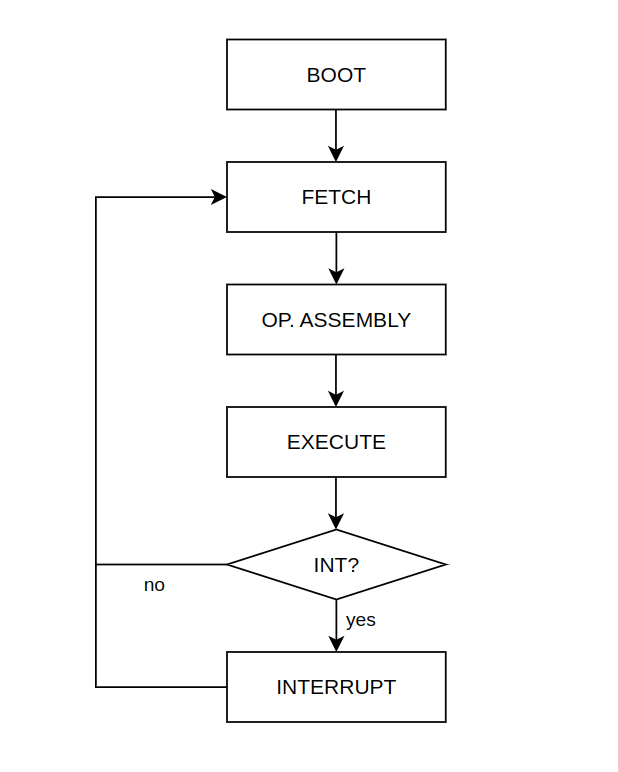
\includegraphics[width=0.5\textwidth]{img/BootInt.png}
    \caption{Ciclo di esecuizone con interrupt}\label{img:bootint}
\end{figure}
Quindi quando le interruzioni sono scatenate vanno ad effettuare una chiamata a subroutine particolare, tale chiamata è detta ISR (Interrupt-Services-Routine). Tale situazione, quindi, ferma il sistema dalla sua normale esecuzione del programma per dare priorità alla gestione dell'interruzione. Questo, quindi, apre molti dubbi su come gestire lo stato in cui si trova la macchina, poichè se quando torno dalla ISR, ho cambiato qualche registro significativo si potrebbe compromettere il normale funzionamento del programma. In generale i due registri che richiedono l'obbligo di essere salvari sono i registri: \textbf{SR(Status register)} e il \textbf{PC(Program Counter)}. In generale, i registri che vado a salvare in questo passaggio sono anche detti: \textbf{Descrittore di processo}, tali registri, quindi, descrivono lo stato di funzionamento del mio processore quando poi è stato prelazionato dalla mia ISR. Ciò mi permette di proseguire ancora con la normale esecuzione del programma prefissato.

\subsubsection{Gestione delle Interruzioni}
Una volta definito cosa sono le interruzioni è di fondamentale importanza capire come il processore le gestisce. Le principali modalità di gestione delle interruzioni sono due e sono:
\begin{itemize}
    \item \textbf{Vettorizzate}: Ogni livello di priorità di interrupt è collegato al processore. I fili di collegamento per le interrupt sono limitati, quindi più dispositivi possono collegarsi sullo stesso cavo di interrupt. Il processore, quindi, per identificare il dispositivo che ha scatenato l'Interrupt va a controllare i bus, su cui il dispositivo ha caricato il suo codice identificativo. Identificare il dispositivo, vuol dire identificare la tipologia di ISR da andare ad utilizzare. Gli indirizzi degli entry-point delle varie periferiche sono memorizzati in memoria a partire dall'indirizzo 0 a seguire per 256 locazioni di 4 byte. Tali locazioni si dividono nel seguente modo:
    \begin{itemize}
        \item \textbf{Funzioni speciali}: Da 0 a 24, gli entry-point identificano delle funzioni speciali o di gestione aritmentica
        \item \textbf{Interruzioni autovettorizzate}: da 25 a 31 sono indicizzate le locazioni per il funzionamento autovettorizzato
        \item \textbf{Trap}: da 32 a 47 sono indicizzate le funzioni per la gestione dei Trap
        \item \textbf{Utilizzabili}: da 48 a 256 sono locazioni disponibili per l'inserimento degli entry-point per la gestione di diverse periferiche
    \end{itemize}
    \item \textbf{Autovattorizzate}: A differenza del caso vettorizzato, evita la lettura del codice identificativo, poichè ogni livello di interrupt è collegato al vettore delle ISR autovettorizzate e permette di selezionare in maniera "ignorante" l'ISR alla locazione della tipologia di priorità inserita
\end{itemize}

\subsubsection{PIC} \label{par:PIC}
In generale, nel caso di sistema \textbf{vettorizzato}, viene in aiuto il componente \textbf{PIC (Programmable Interrupt Controller)} [\ref{img:PIC}].
Il PIC è un dispositivo che permette di arricchire le
modalità di gestione delle interruzioni. Grazie alla programmazione di questo oggetto, possiamo assegnare alle varie periferiche non una sola linea di interruzione con una specifica ISR, ma possiamo esplorare tutto il vettore delle interruzioni, che in teoria è costituito da 256 locazioni. In sostanza, il PIC permette di usare \textbf(interrupt vettorizzate), ovvero il dispositivo fornisce sul data bus un vettore di 8 bit che rappresenta l’indice all’interno della tabella delle interruzioni corrispondente all’indirizzo della corretta ISR. Nel M68k questo protocollo è simulato con il PIC: Il dispositivo non scrive sul data bus il vettore di 8 bit, ma comunica l’interruzione al PIC che si occuperà di capire qual è il vettore corrispondente al dispositivo interrotto. Il PIC estende la gestione delle interruzioni del processore M68K introducendo nuove funzionalità, come la gestione prioritaria, la mascheratura delle interruzioni e le linee di interrupt. Il dispositivo ha in uscita verso il processore una linea di interruzione INT e una linea di INTA (acknowledgement) , mentre ha in ingresso 8 linee di interruzioni differenti, a priorità decrescente (0 massima, 7 minima).

\begin{figure} [h!]
    \centering
    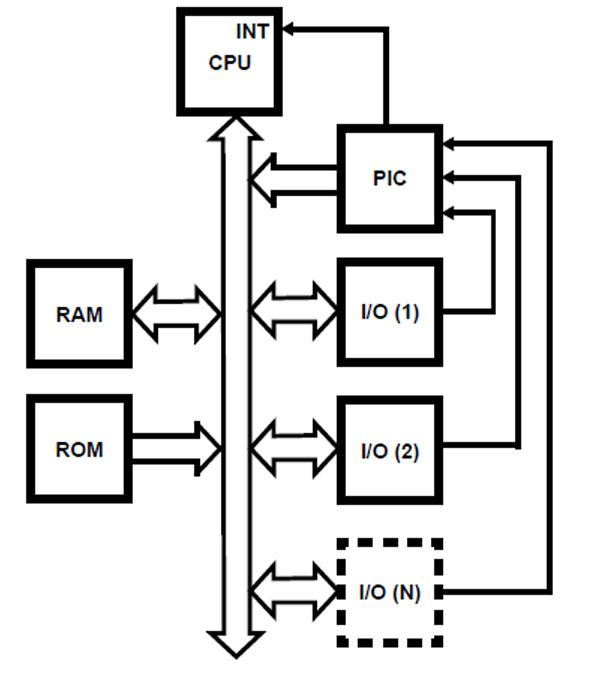
\includegraphics[width=0.5\textwidth]{img/PIC3.png}
    \caption{PIC}\label{img:PIC}
\end{figure}

Nella trattazione del PIC faremo riferimento ad un particolare chip, lo \textbf{82C59A} \ref{img:82C59A}, per la sua particolare compatibilità. Un singolo PIC può gestire fino a 8 livelli di priorità, ma è possibile creare un sistema di PIC in cascata per arrivare a gestire fino a 64 livelli di priorità. 

% Più dispositivi possono essere connessi in cascata, fino a 8 per un massimo di 64 linee di interruzione.
% Il PIC accetta richieste di interruzione dai dispositivi di IO connessi alle sue linee e determina, a seconda dell’algoritmo di gestione prioritaria selezionato, quale delle interruzioni simultaneamente attiva ha la priorità più alta. Dopodiché trasmette un segnale sulla linea INT al processore, attende un segnale su INTA (handshaking) e poi trasmette sul bus dati il vettore di 8 bit a cui corrisponde la corretta interruzione sulla tabella delle interruzioni.
% Il Control Register interno al PIC permette di configurare la gestione prioritaria mediante un’opportuna modifica:
Il PIC prevede due modalità di gestione delle priorità:
\begin{itemize}
    \item \textbf{Fully nested mode}: le richieste di interruzione sono ordinate secondo uno schema a priorità fissa che va da IR0 a IR7, con IR0 la linea più prioritaria;
    \item \textbf{Rotate mode}: Schema prioritario a rotazione (Round robin), ovvero la linea di interruzione più prioritaria appena servita diventa la meno prioritaria dopo il servizio. Da programma è possibile configurare il livello di priorità più basso.
    % \item \textbf{Maschera interruzioni} consente l’inibizione o l’abilitazione delle linee di interruzione. 
\end{itemize}

Osservando i componenti interni in figura \ref{img:82C59A}, notiamo i seguenti componenti:
\begin{itemize}
    \item \textbf{IRR}: Interrupt request register, ovvero un registro di 8 bit per ciascuna linea di interruzione in ingresso, finalizzato a memorizzare le richieste di interruzione;
    \item \textbf{ISR}: In service register, registro che memorizza i livelli di interruzione correntemente serviti;
    \item \textbf{Priority Resolver}: componente che determina le priorità delle richieste memorizzate dall'IRR e decide \textit{quale} istruzione deve essere servita, ovvero quale bit dell' ISR settare.
    \item \textbf{IMR}: Interrupt Mask Register, registro che contiene una maschera che serve a disabilitare selettivamente una o più linee di interruzione;
    \item \textbf{Bloccho R/W control}: Il blocco riceve i comandi dalla CPU per la configurazione del dispositivo e permette di “leggerne” lo stato interno;
    \item \textbf{Cascade buffer comparator}: viene utilizzato quando il PIC è collegato ad altri PIC in cascata, e le linee connesse a questo blocco servono a regolare la logica PIC master/slave.
\end{itemize}

\begin{figure}[h!]
    \centering
    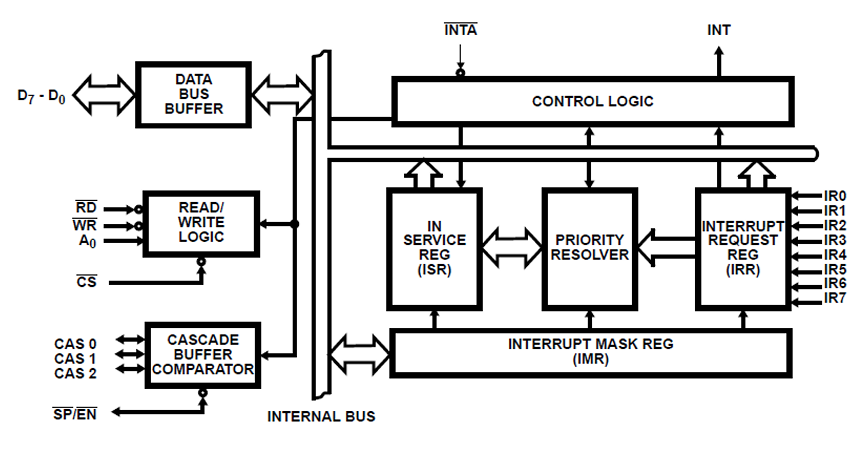
\includegraphics[width=1\textwidth]{img/PIC_82C59A.png}
    \caption{82C59A}
    \label{img:82C59A}
\end{figure}

Procediamo illustrando la modalità di funzionamento:
Inizialmente, uno o più dispositivi connessi al PIC inviano un'interruzione sulla linea alla quale sono connessi. La richiesta che arriva sulla linea i-esima, pone a 1 l'i-esimo bit del registro \textbf{IRR}. A questo punto, il \textbf{priority resolver} decide quale dispositivo deve essere servito sulla base delle priorità associate ad ogni dispositivo e in base al contenuto dell'\textbf{IMR}, e inoltra una richiesta di interruzione alla CPU (o ad un altro PIC cui è connesso in cascata) tramite la linea INT. La CPU a questo punto invia un ACK sulla linea INTA per segnalare eventualmente la disponibilità a servire l'interruzione. 
Una volta ricevuto l'ACK, il PIC setta il bit del registro \textbf{ISR} corrispondente alla linea interrompente a maggiore priorità, e resetta il corrispondente bit del registro \textbf{IRR}. Il PIC a questo punto trasmette sul \textit{bus dati} il vettore relativo al dispositivo interrompente e il bit del registro ISR corrispondente al dispositivo viene resettato. Questo ultimo reset può avvenire in due modalità:
\begin{itemize}
    \linespread{0.4}
    \item \textit{automaticamente}, se è stata selezionata la modalità \textit{automatic end of interrupt};
    \item \textit{manualmente}, settando un bit opportuno EOI tramite una parola di controllo appena prima di uscire dalla ISR.
\end{itemize}

Attraverso i blocchi \textbf{Data Bus Buffer} (linee D0-D7) e \textbf{R/W logic} (linea !RD, !WR, A0, !CS) è possibile accettare due tipi di command word proveniente dalla CPU:
\begin{itemize}
    \item \textbf{ICW}s: Initialization Command Words, che servono ad \textit{inizializzare} il dispositivo con una sequenza di minimo due e massimo quattro comandi di inizializzazione.
    \begin{itemize}
        \item \textbf{ICW1}: identificato da (A0=0,D4=1), inizia la sequenza di inizializzazione resettando il dispositivo e impostando alcuni parametri di configurazione, attraverso gli altri bit Dx.
        \item \textbf{ICW2}: segue la ICW1, identificato da A0=1, specifica i bit di indirizzo per localizzare la tabella dei vettori delle interruzioni in base al tipo di processore selezionato con la ICW1 ( 8080/85 o 80C86/88/286);
        \item \textbf{ICW3}: Identificata da A0=1, questa parola viene letta solo quando c'è più di un 82C59A in cascata, informazione acquisita attraverso la ICW1.
        \item \textbf{ICW4}: Identificata da A0=1, viene usato se in ICW1 è stato specificato IC4=1. Consente di specificare se il dispositivo deve funzionare in special fully nested mode o in buffered mode, il tipo 
        di processore con cui deve interfacciarsi, e se bisogna abilitare l'automatic end of interrupt (\textbf{AEOI}).
    \end{itemize}
    \item \textbf{OCW}s: Operation Command Words, servono a configurare la modalità di funzionamento.Dopo aver inizializzato il dispositivo con le ICW, esso è pronto ad accettare richieste di interruzione e può essere configurato con ulteriori parametri operativi:
    \begin{itemize}
        \item \textbf{OCW1}: Setta e resetta i bit della maschera nell'IMR.
        \item \textbf{OCW2}: consente di configurare il funzionamento del dispositivo per quanto riguarda la modalità \textit{end of interrupt} (permette di resettare in maniera programmatica il bit nel registro ISR) e \textit{rotate} (permette di specificare il meccanismo di rotazione delle priorità man mano che le interrupt su una linea vengono servite).
        \item \textbf{OCW3}:  consente di attivare/disattivare la special mask mode, in cui è possibile mascherare  “temporaneamente” uno specifico livello di richiesta senza avere effetto sui livelli più bassi o più alti. Il livello da mascherare è quello specificato in precedenza nella OCW1.
    \end{itemize}
\end{itemize}


Dal punto di vista esercitativo, al corso è stato presentato un componente da utilizzare nel framework ASIM che rappresenta una versione estremamente semplificata del PIC, il cui schema logico è raffigurato in figura \ref{img:piceasy}.
Il device simulato presenta 8 linee di richiesta, a ciascuna delle quali è associata una priorità fissa (modalità \textit{fully nested}), a cui possono essere connessi fino a 8 dispositivi con 8 livelli di priorità, stabiliti mediante lo schema \textit{daisy chain}. 
Il modello di programmazione del dispositivo occupa due locazioni consecutive di memoria e prevede 5 registri accessibili al programmatore. \\


\begin{tabular}{|p{3cm}|p{10cm}|}
    \hline
    \centering \textbf{IMR} &  (Interrupt Mask Register) permette di mascherare singolarmente le interruzioni \\
    \hline
    \centering \textbf{IRR} &  (Interrupt Request Register): memorizza i segnali di interruzione \\
    \hline
    \centering \textbf{ISR} &  (In Service Register): presenta al gestore delle interruzioni i segnali interrompenti in modo ordinato rispetto alla maschera e alla priorità corrente \\
    \hline
    \centering \textbf{CTRL} &  (Control Register): permettere di controllare il comportamento del dispositivo\\
    \hline
    \centering \textbf{TR} &  (Type Register): memorizza la parte base dell’indirizzo del vettore \\
    \hline
\end{tabular}


% Il modo di operazione scelto deve essere configurato in fase di inizializzazione del PIC, ma può anche essere dinamicamente cambianto da un apposito programma di gestione. Per i registri interni al PIC facciamo riferimento alla figura \ref{img:PIC2}.
% L’Interrupt Request Register (IRR) riceve in ingresso le 8 linee di interruzione provenienti dalle periferiche collegate e ne memorizza lo stato. L’input a questo registro è gestito da un circuito integrato che si occupa della gestione prioritaria delle interruzioni, mentre l’output è il registro In Service Register (ISR) in cui vengono memorizzati solo i segnali di interruzione da servire in accordo alla maschera (IMR). Il Type Register (TR) è un registro di 8 bit che memorizza nei 5 bit più significativi il valore base del vettore da scrivere in output sul bus dati, mentre nei 3 meno significativi uno spiazzamento in accordo alla linea interrompente. Dopo il servizio, l’i-esimo bit di IRR è automaticamente cancellato per riuovere la causa di interruzione.


% \begin{figure}
%     \centering
%     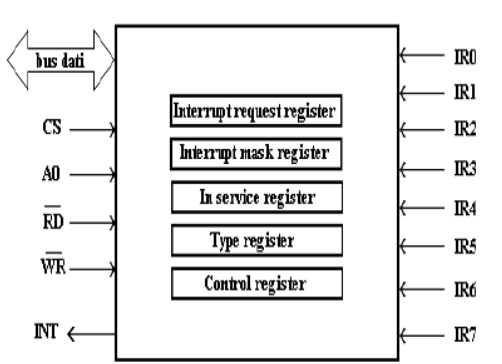
\includegraphics[width=0.5\textwidth]{img/PIC2.png}
%     \caption{PIC: modello di programmazione}\label{img:PIC2}
% \end{figure}


\begin{figure}[!ht]
    \centering
    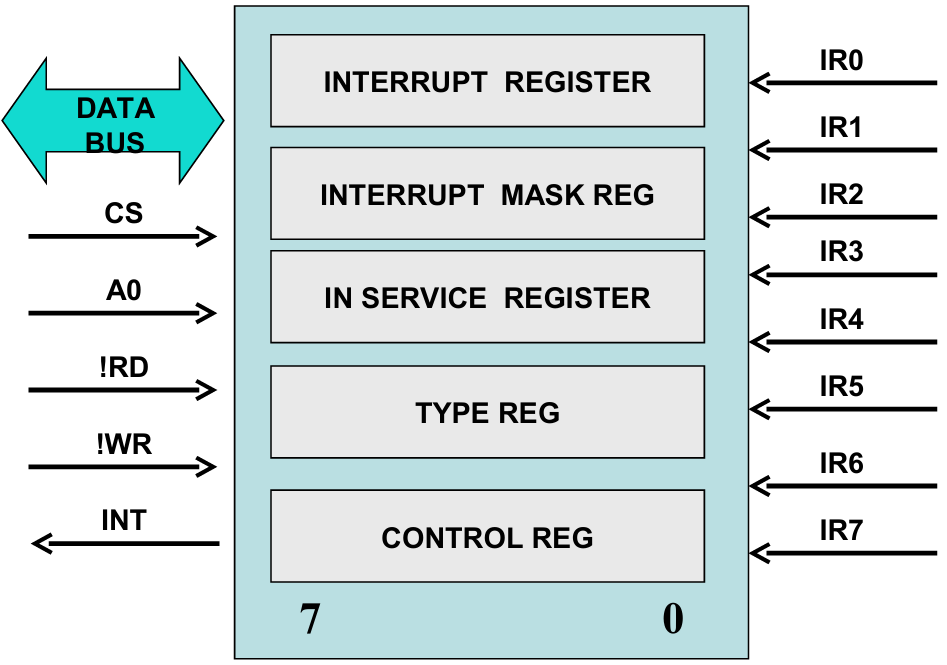
\includegraphics[width=0.7\textwidth]{img/easy_pic.png}
    \caption{PIC semplificato}
    \label{img:piceasy}
\end{figure}

Vediamo nel dettaglio il funzionamente di questi registri:
\begin{itemize}
    \item \textbf{TYPE REGISTER}: contiene informazioni sui vettori di interruzione associati al PIC. I vettori si ricavano a partire da un \textit{vector number} di base sommando uno spiazzamento su 3 bit, ovvero i 3 bit meno significativi del registro. Lo spiazzamento viene settato automaticamente in base alla linea interrompente. Praticamente al programmatore è permesso di inserire il numero di base, al quale viene automaticamente sommato uno spiazzamento in base alle linea interrompente.  L’accesso a TR viene fatto selezionando in scrittura  l’indirizzo dispari subito dopo un textit{RESET};
    \item \textbf{INTERRUPT MASK REGISTER}: memorizza le linee di interruzione che devono essere mascherate. Per mascherare una linea basta inserire un 1 nel bit corrispondente. IMR è accessibile sia in lettura che in scrittura ad indirizzo dispari, ma in scrittura il dispositivo non deve essere nello stato \textit{reset}, ovvero deve essere già stato scritto almeno TR;
    \item \textbf{CONTROL REGISTER}: registro da 8 bit accessibile sempre in scrittura ad indirizzo pari:
    \begin{itemize}
        \item bit 0,1,2: determinano il bit da cancellare in \textit{ISR}.
        \item bit 3: bit End of Interrupt, se posto a 1 fa cancellare il bit puntato dai bit 0-2. 
        \item bit 4: bit Automatic End of Interrupt, se posto a 1 fa cancellare automaticamente il bit in ISR dopo la trasmissione dell'interruzione;
        \item bit 5: \textit{non utilizzato};
        \item bit 6: bit Register Interrupt Selector, se il bit 7 è alto seleziona l'accesso a ISR in lettura, se il bit 7 è basso seleziona l'accesso a IRR in lettura;
        \item bit 7: permette se posto a 1 la lettura dei registri ISR e IRR (vedi punto precedente).
    \end{itemize}
    \item \textbf{INTERRUPT REQUEST REGISTER}: memorizza le richieste di interruzione relative alle singole linee di interruzione. Questo registro è accessibile solo in lettura ad indirizzo pari in accordo a quanto scritto nel registro CTRL. 
    Quando la richiesta d'interruzione, arrivata sulla linea n, viene spedita al gestore delle interruzioni (PIC o CPU) collegato al PIC, il bit n-esimo di IRR è cancellato;
    \item \textbf{IN SERVICE REGISTER}: sono memorizzate le interruzioni trasmesse.  Questo registro è accessibile solo in lettura all'indirizzo pari in accordo con quanto settato nel registro di controllo. 
\end{itemize}

\subsection{Estensione del modello IO generale}
Un modello di architettura dotato solo di PIA (\ref{par:PIA}) è limitato: può gestire solo caratteri, ha a disposizione solo 7 interruzioni e può generare attese infinite con il protocollo di handshaking.
Per risolvere questi problemi, vengono introdotti nuovi elementi nell'architettura: \textbf{DMA} per gestire il trasferimento di messaggi invece di caratteri, \textbf{PIC} (\ref{par:PIC}) per superare la limitazione sul numero di ISR indirizzabili e \textbf{TIMER} per gestire la temporizzazione e il risolvere il problema delle attese infinite (\ref{img:IO_ESTESO}).

\begin{figure}[h!]
    \centering
    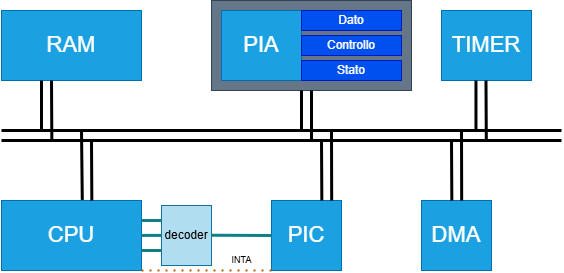
\includegraphics[width=0.75\textwidth]{img/Schema_IO_1.png}
    \caption{Modello IO esteso - schema logico}
    \label{img:IO_ESTESO}
\end{figure}

Il timer espone il modello di programmazione Registro di stato, Registro di valore e Registro di Modo. Nel registro di valore di solito è scritto un istante in cui il timer si "sveglia" e genera un'interruzione: infatti il timer possiede una linea con la quale può comunicare un'interruzione.
